\nonstopmode
\documentclass{beamer}
%
% Choose how your presentation looks.
%
% For more themes, color themes and font themes, see:
% http://deic.uab.es/~iblanes/beamer_gallery/index_by_theme.html
%
\mode<presentation>
{
  \usetheme{default}      % or try Darmstadt, Madrid, Warsaw, ...
  \usecolortheme{default} % or try albatross, beaver, crane, ...
  \usefonttheme{default}  % or try serif, structurebold, ...
  \setbeamertemplate{navigation symbols}{}
  \setbeamertemplate{caption}[numbered]
} 

\usepackage{amsmath}
\usepackage[english]{babel}
\usepackage[utf8]{inputenc}
\usepackage[T1]{fontenc}
\usepackage{unicode-math}
\usepackage{tikz}
\usetikzlibrary{matrix}
\usetikzlibrary{calc}
\usetikzlibrary{fadings}
\usetikzlibrary{arrows,automata}
\usetikzlibrary{intersections}

\title[Temporal/FraCaS]{Applied Temporal Analysis: A Complete Run of the FraCaS Test Suite}
\author{Jean-Philippe Bernardy and Stergios Chatzikyriakidis}
\institute{CLASP, University of Gothenburg}
\date{IWCS 2021}

\newcommand\ConId[1]{\mathsf{#1}}


\begin{document}

\begin{frame}
  \titlepage
\end{frame}


\begin{frame}
  \begin{itemize}
  \item 
    Our starting point is the FraCoq system (Presented by the same authors at IWCS 2017 with updates at NoDaliDa 2019):
    
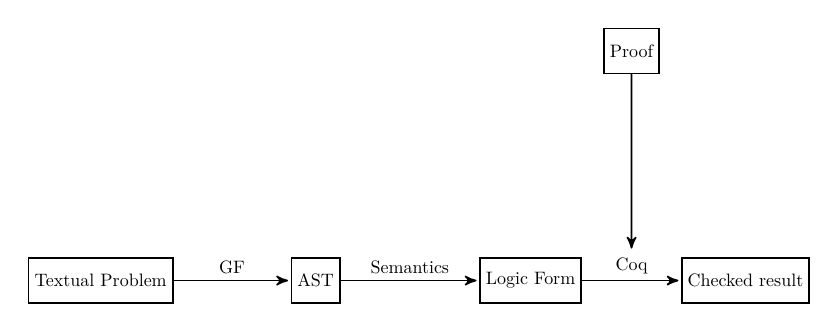
\begin{tikzpicture}[->,>=stealth',shorten >=1pt,auto,node distance=4.2cm,
                    semithick,scale=0.65, every node/.style={transform shape}]
  \tikzstyle{every state}=[draw=black,text=black,shape=rectangle]

 \node[state]         (txt)                {Textual Problem};
 \node[state]         (ast) [right of=txt] {AST};
 \node[state]         (pp)  [right of=ast] {Logic Form};
 \node[state]         (math)    [right of=pp]  {Checked result};

 \path (txt) edge              node (GF)  {GF}                  (ast)
       (ast) edge              node (Hask) {\alert{Semantics}} (pp);
 \path  (pp) edge               node (Coq) {Coq} (math);

 \node[state]         (proof) [above of=Coq]  {Proof};
 \path  (proof) edge                (Coq);
       
\end{tikzpicture}
\item
In this paper we update the \alert{Semantics} with {Temporal Semantics}. We achieve coverage of 329 out of 337 problems in the FraCaS test suite, with an accuracy of 81\%.
  \end{itemize}
\end{frame}

\begin{frame}

\begin{itemize}
  \item (Smith wrote a novel in 1991 $⇒$ Smith wrote it in 1992) is false
    \begin{itemize}
    \item \[\begin{array}{l}
∀x. \ConId{novel}(x) ∧ \\
∃t_1,t_2.  [t_1,t_2] ⊆ 1991 ∧ \ConId {write}(\ConId{smith},x,t_1,t_2) ∧ \\
∃t_3,t_4.  [t_3,t_4] ⊆ 1992 ∧ \ConId {write}(\ConId{smith},x,t_3,t_4) \\
⟶ ⊥
\end{array}
\]
is provable
\end{itemize}
\item (Smith wrote a novel in 1991 $⇒$ Smith wrote a novel in 1992.) is neutral


  \begin{itemize}
  \item \[\begin{array}{l}
(∃x. \ConId{novel}(x) ∧ \\
∃t_1,t_2. [t_1,t_2] ⊆ 1991 ∧ \ConId{write}(\ConId{smith},x,t_1,t_2)) → \\
(∃y. \ConId{novel}(y) ∧ \\
∃t_3,t_4. [t_3,t_4] ⊆ 1992 ∧ \ConId{write}(\ConId{smith},y,t_3,t_4)) \\
 \\
\end{array}
\]
is not provable.
\end{itemize}
\end{itemize}

\end{frame}


\end{document}

